\section{POODLE}

\subsection{概要}
SSL 3.0 は,1995年に発表された旧式の暗号化プロトコル.
POODLEとは,Padding Oracle On Downgraded Legacy Encryptionの頭文字をとったもので,SSL3.0において,ブラウザが暗号化を処理する仕組みに存在する脆弱性をPOODLE脆弱性という.2014年10月に発見された.

\subsection{脆弱性の内容}
パディングとは,平文をブロックに分けて暗号化を行なうブロック暗号方式などにおいて,データを固定長として扱いたいときに,短いデータの前や後に無意味なデータを追加して長さを合わせる処理のことである.パディングは,プロトコルによって検証されないため,攻撃者は任意データをパディングとして利用する.また,攻撃者は,TLS/SSLのバージョンをダウングレードすることが可能で,SSL 3.0における暗号化通信で,リクエスト送信を繰り返し試み,1つ前のデータを繰り返し推測することで,暗号化された通信を1バイトずつ平文に復号し,入手可能になる.\cite{mobage}
SSL3.0において,暗号文がちょうどブロック長の倍数の長さのときでもパディングを設ける必要がある.攻撃者は,中間者攻撃を行うが,暗号を直接的に復号することは行わず,クライアントから送信された暗号文自体を細工してサーバに送りサーバ側での処理結果を確認するという手法を用いる.
SSL3.0では,CBC方式のブロック暗号(図1)を用いる.平文の最後がブロック長に比べて途中で終わってしまった場合,はみ出た部分にダミーの文字を入れて,ブロックサイズの倍数に揃うように調整する.この文字をパディングという.平文の一番最後のバイトにパディングの長さが入るようになる.復号した際に,後ろからパディングの長さ分の文字を無視することで元の平文を取得可能になる.この時に,一番最後のバイトはパディング長として規定されているため,平文が丁度ブロックサイズの倍数であっても,パディング長情報のbyte分がはみ出てしまうため,その場合は,最後のブロックはダミーの文字とパディング長のみの実質データが入っていないようなブロックになる.(図2)
POODLEでは,パディングのみで構成されているブロックを悪用し,他のブロックの平文の推測を行う.SSL3.0のパディング方式では,ダミーの文字部分は無視され,パディング長さのみ正しいことが要求される.したがって,パディングのみで構成されているブロックの暗号文が改ざんされても,復号を行った結果の最後のバイトが正しいパディング長のバイトと一致した場合,正しい暗号文として扱われる.つまり、おおよそ1/256の確率(1byteが偶然一致する確率)で、暗号文が復号された結果の最後のbyteがパディングと同じになるということが判別可能になる.この判別結果を利用することで、後述の手法により任意の暗号ブロックの最後のbyteの復号結果を検証することが可能になる.まず,クライアントからの同じ通信内の他の暗号ブロックをパディングのブロックにブロックごと上書きしてサーバに送信することで,該当のブロックの復号結果を見る.(図3)攻撃者はクライアントに同じデータを送信させて,同様の手法を繰り返し行うことで偶然復号結果のパディング長に相当する最後のbyte部分が一致する場合がある(1/256の確率).\cite{trend}
一致した場合には,図4のような手順で復号する.


\begin{figure}[h!]
\begin{center}
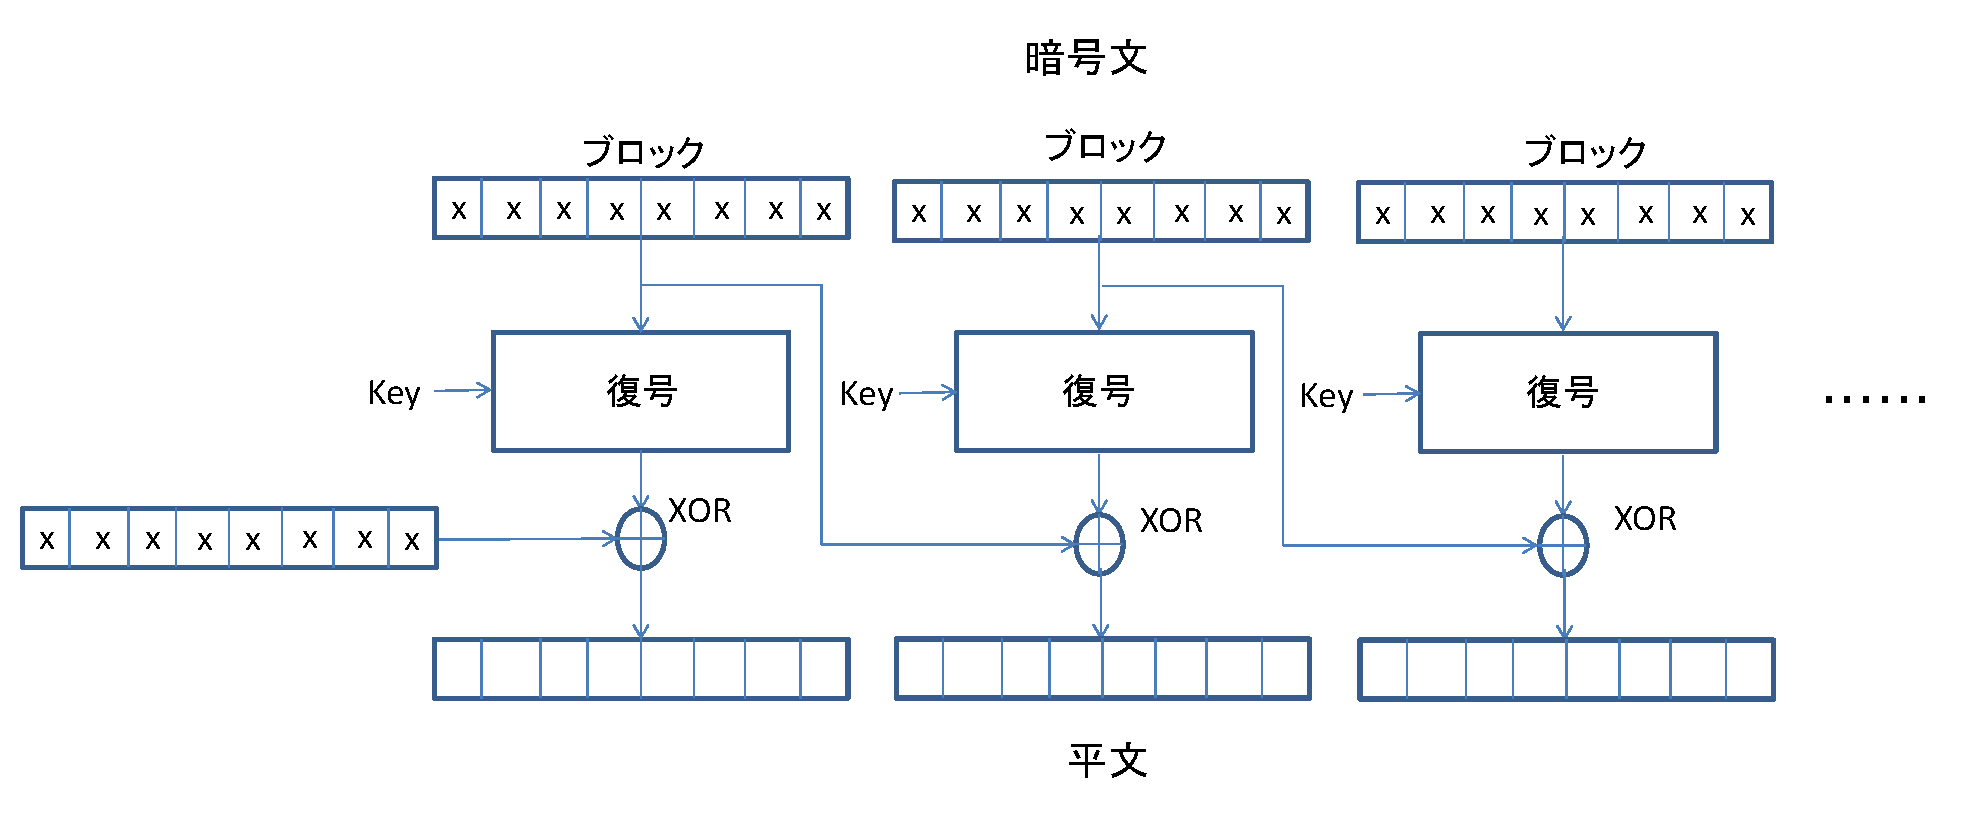
\includegraphics[scale=0.4]{1poodle.eps}
\caption{ブロック暗号の復号処理}
\end{center}
\end{figure}

\begin{figure}[h!]
\begin{center}
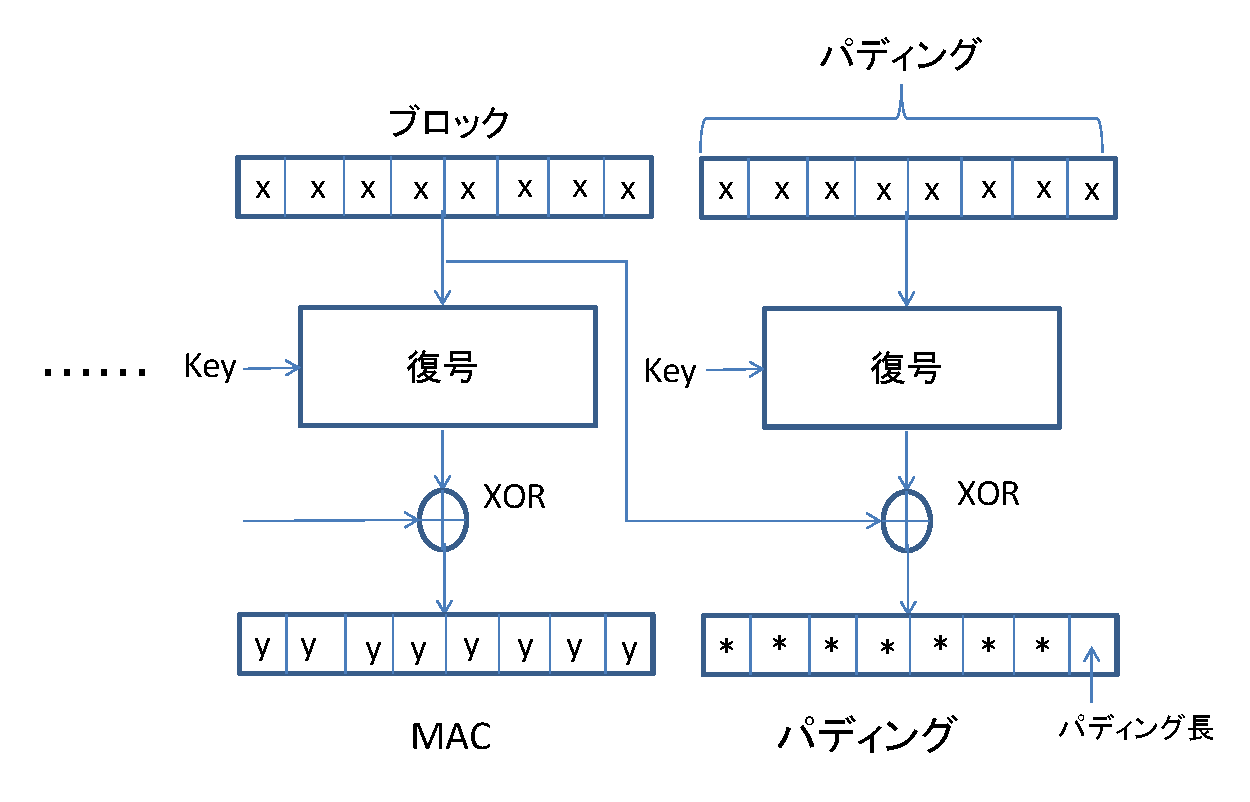
\includegraphics[scale=0.4]{2poodle.eps}
\caption{最後のブロックがパディングのみになった場合の復号例}
\end{center}
\end{figure}

\begin{figure}[h!]
\begin{center}
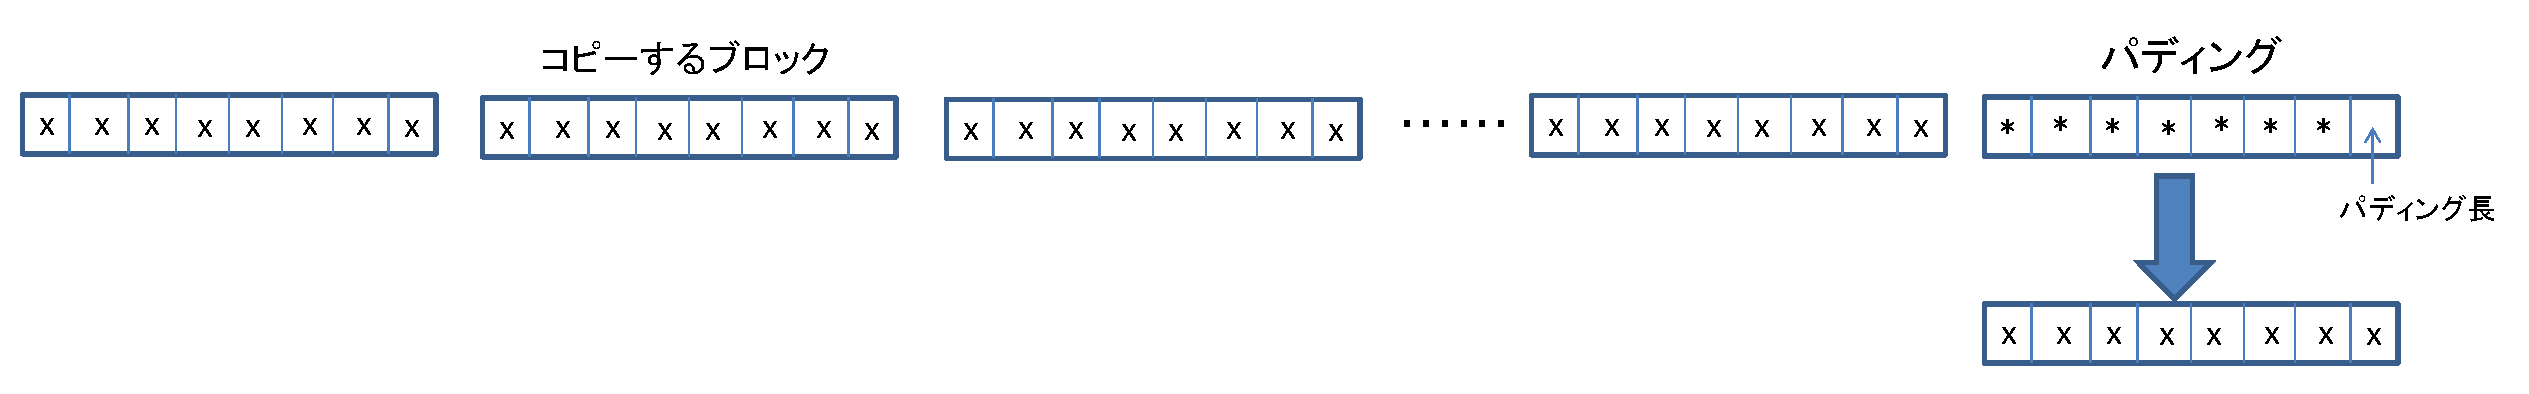
\includegraphics[scale=0.4]{3poodle.eps}
\caption{暗号文の変更}
\end{center}
\end{figure}

\begin{figure}[h!]
\begin{center}
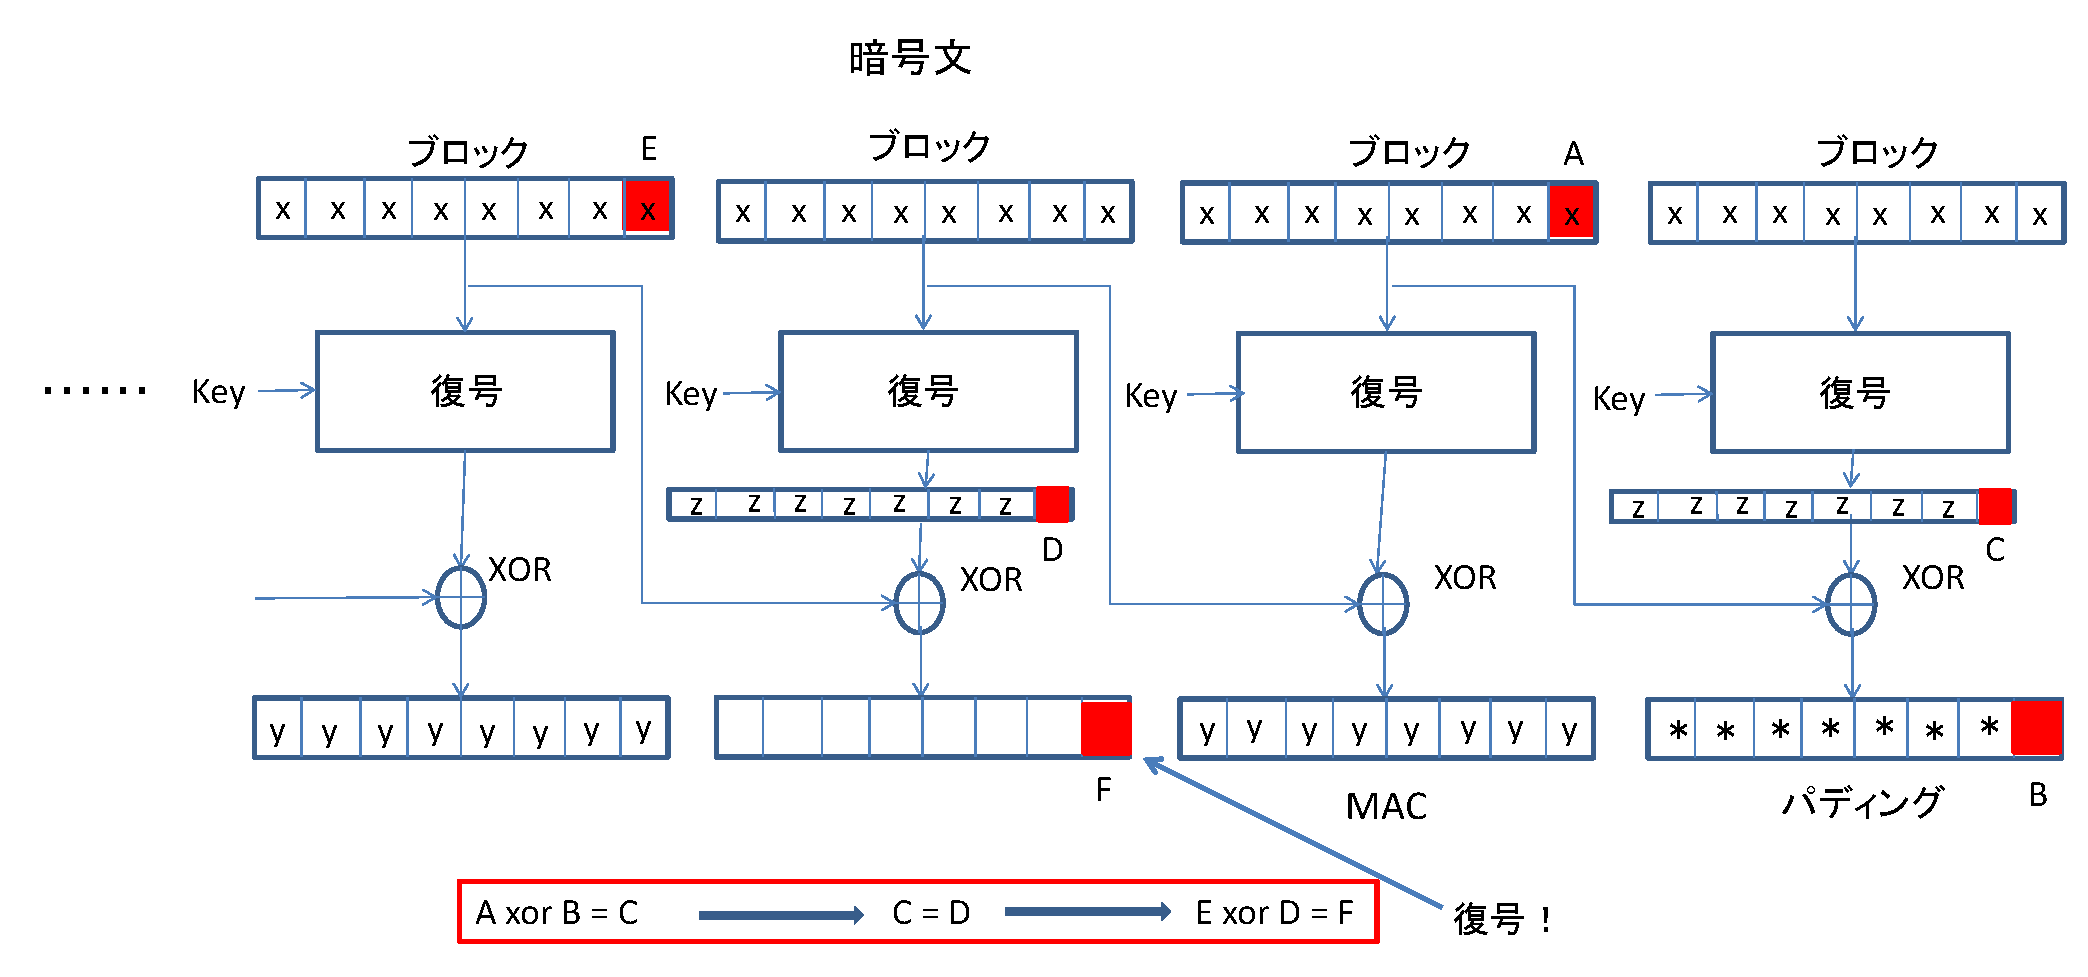
\includegraphics[scale=0.4]{4poodle.eps}
\caption{復号手順}
\end{center}
\end{figure}

\subsection{対策}
ブラウザ,webサーバーともに,SSL 3.0を無効にする.
